Quantum computers are devices that exploit the features of quantum mechanics at
the smallest scales of reality. They even have the potential to solve
computational problems that are not feasible for conventional computers
\cite{nielsen_chuang_2010}. Some of the most famous applications are the
accurate simulation of physics \cite{feynman82_simul_physic_with_comput}, fast
database searching provided by Grover's algorithm \cite{Grover_1996} and the
polynomial time solution for factoring large composite numbers, provided by
Shor's algorithm \cite{Shor_1997}, which has far-reaching consequences for
current methods in cryptography. However, there are still key technological
challenges that need to be overcome before this technology can be realized.

To date, superconducting LC circuits have shown the greatest promise in forming
effective quantum bits (or qubits) \cite{Rol_2019}
\cite{barends14_super_quant_circuit_at_surfac}, however several other platforms,
such as quantum dots \cite{huang19_fidel_bench_two_qubit_gates_silic}
\cite{Lawrie_2020}, NV-centres in diamond \cite{Taminiau_2014}, and even
topological qubits in semi-conducting nanowires \cite{Mourik_2012}, have seen
growing interest and recent development. Nevertheless, they all suffer from some
form of noise, of a slightly different nature in each case, which poses
major challenges in the realization of a scalable quantum computer.

Accounting for this noise is undoubtedly a daunting task. For that, different
approaches have been developed which are usually grouped as part of
\textit{quantum error suppression} (QES), such as dynamical decoupling, which
attempt to reduce the noise at the hardware level, and \textit{quantum error
  correction} (QEC) techniques, which aim to correct errors once they have
occurred. In particular, the latter approach has undergone rapid development in
recent decades from the schemes proposed by Shor \cite{Shor_1995_QEC} and Steane
\cite{Steane_1996_QEC} to the new promising \textit{surface codes}
\cite{fowler12_surfac_codes} that have higher tolerance to errors and require
fewer interactions among the qubits.

In this article, we review the key principles of quantum error correction,
discuss ...

\subsection{Principles of Quantum Error Correction}
% I think that here we should mention what the [[n,k,d]] code is.
In the basic theory of quantum error correction, quantum states are encoded into
several physical qubits. By performing the appropriate parity checks, it is
possible to probe the state of the encoded qubit (which is comprised of many
physical qubits) without changing its state, in order to detect errors on
individual physical qubits. These parity checks are the \textit{stabilizers} of
the QEC code; when all stabilizer measurements return an eigenvalue
of $+1$, it signals that no error has occurred \cite{nielsen_chuang_2010}.
Effective encoding protocols are such that each error process gives rise to a
unique syndrome, which is just the list of stabilizer measurement outcomes,
which provides the information needed to correct the error \cite{fowler12_surfac_codes}.

\begin{figure}
  \centering
  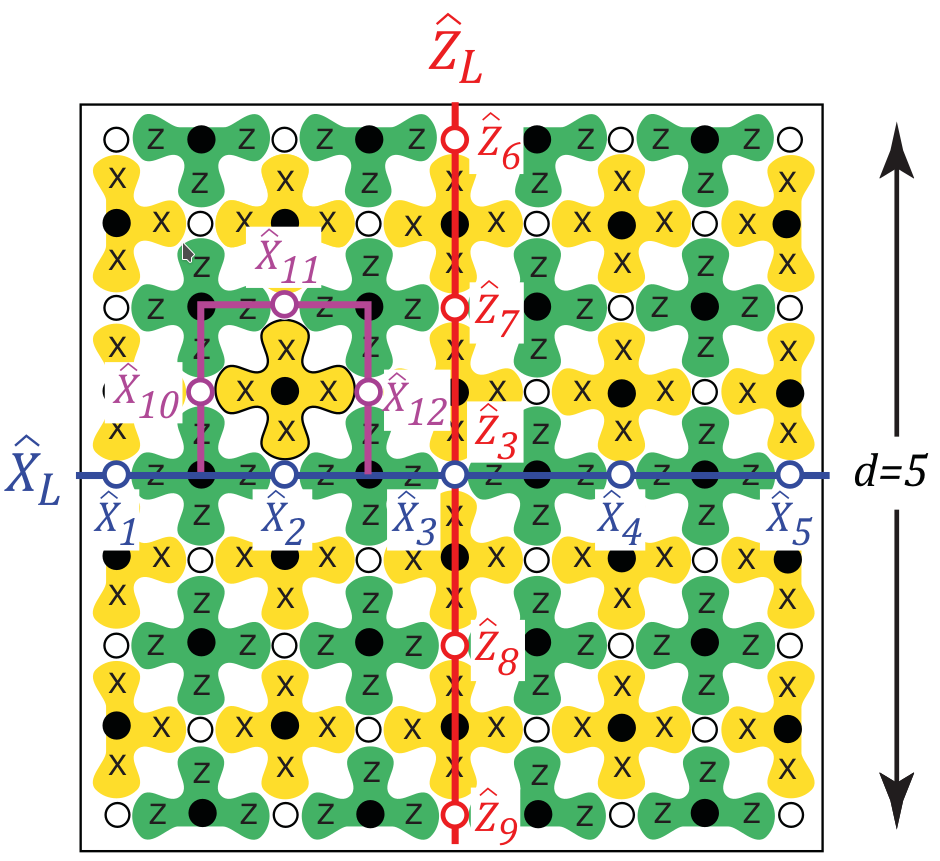
\includegraphics[width=0.4\textwidth]{images/surface_code.png}
  \caption{A 2D array of qubits implementing the surface code. Data qubits are
    the white circles, which are connected to 2 $Z$- and 2 $X$-stabilizers
    respectively. This code is capable of precisely characterizing Pauli noise
    due to the complimentary spacing of the $X$ and $Z$ checks. Figure from
    \cite{fowler12_surfac_codes}.}
  \label{fig:surface_code}
\end{figure}

In any real implementation of physical qubits, there are several sources of
error. State preparation and measurement may not be carried out perfectly.
Coherent errors also occur through the imperfect application of quantum gates in
circuits \cite{Devitt_2013}. Error models and QEC schemes are all
predicated on the assumption that low-weight errors (affecting only a few
qubits) are more likely than high weight errors. In other words, error
probabilities must be small \cite{terhal15}. In principle though, all these
(small) sources of error can be corrected for using a variety of encoding and
detection schemes.

The error detection scheme implemented by the surface code, shown in Fig.
\ref{fig:surface_code}, is capable of precisely identifying errors in large
arrays of qubits. The $X$- and $Z$-stabilizer ancillas conduct parity
measurements between the data qubits to which they are connected through a
sequence of CNOT operations. Should an error occur on a given data qubit,
depending on the error type ($X$, $Y$, or $Z$) either the $X$ or $Z$ (or both)
type stabilizers will fire (return an outcome of $-1$ in their measurement),
alerting us to the error.

One great strength of the surface code is its ability to diagnose multiple
errors simultaneously. Should two adjacent $X$-checks fire at one end of the
surface, while two $Z$-checks fire at the other end, we can conclude that a
phase-flip error occurred on the data qubit between the two $X$-checks, while a
bit-flip error occurred between the $Z$-checks. One must be careful, however,
because decoding the error syndrome for any code is a problem without a unique
solution \cite{terhal15}. Taking the top-left data qubit in Fig. \ref{fig:surface_code} as an
example, one can confirm that a bit-flip error on that qubit would give rise to
the exact same syndrome as a series of bit-flip errors on the rest of the top
row of data qubits. For systems with small error probabilities, the single
bit-flip error is of course much more likely than the long series of errors
required to produce the same syndrome, but as the error rate grows, such
mistakes in identifying the cause of a syndrome become more commonplace. 

When a syndrome is misinterpreted, the code implements the \textit{wrong
  correction}, and this can lead to a logical level operation being applied to
the logical qubit. The rate at which this occurs, called the \textit{logical
  error rate}, as a function of the physical error rate of the code is of great
interest in characterizing the effectiveness of an error correction protocol.


%%% Local Variables:
%%% mode: latex
%%% TeX-master: "QEC_paper"
%%% End:
